\documentclass{beamer}
\usepackage[italian]{babel}
\usetheme{Berkeley}
\usepackage{graphicx}
\usepackage{booktabs}

\title{PineSU}
\subtitle{Sviluppo di un'applicazione distribuita su Blockchain Ethereum}
\author{Paolo Speziali}
\institute{Università degli Studi di Perugia - Dipartimento di Ingegneria\\[\medskipamount]
      
\includegraphics[width=0.15\textwidth,height=0.15\textwidth]{figures/logo_unipg.png}%
 }
\logo{
\includegraphics[height=1cm]{figures/favicon.png}}
\date{A.A. 2020/2021}

\begin{document}
\begin{frame}
	\titlepage % beamer's \maketitle
\end{frame}
\section{Brainstorming}
\begin{frame}
	\frametitle{Fase 1: Brainstorming}
	Nella scelta dell’attività di tirocinio si è partiti dall’idea di poter unire le funzionalità peculiari delle applicazioni distribuite su Blockchain Ethereum (anche chiamate \emph{DAPP}) assieme a quelle del software di controllo di versione distribuito Git.
	\begin{columns}
		\column{0.5\textwidth}
		\begin{figure}
			
\includegraphics[width=1\textwidth]{figures/ethereum.png}
		\end{figure}
		\column{0.5\textwidth}
		\begin{figure}
			
\includegraphics[width=0.55\textwidth]{figures/git.png}
		\end{figure}
	\end{columns}
\end{frame}
\begin{frame}
	\frametitle{Fase 1: Brainstorming}
	Il pensiero del professore-tutor è andato verso il classico problema presente sia nella pubblica amministrazione sia nelle aziende private di dover controllare l’integrità di file per concorsi o bandi in modo che, una volta registrati, non possano essere manomessi.
	\medskip
	\begin{figure}
		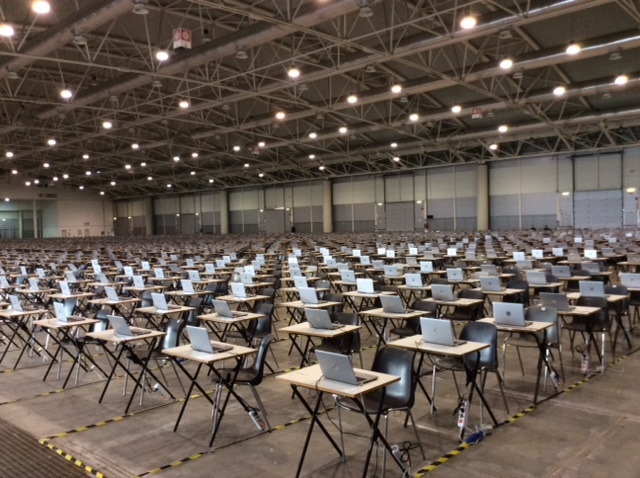
\includegraphics[width=0.40\textwidth]{figures/concorso-fiera-di-roma.jpg}
		\caption{Un concorso pubblico con elaborati digitali}
	\end{figure}
\end{frame}
\section{Specifica dei requisiti}
\begin{frame}
	\frametitle{Fase 2: Specifica dei requisiti}
	Partendo da questa idea lo step successivo è stata la definizione dei requisiti del progetto. Abbiamo perciò concordato che l’attività potesse orientarsi verso la creazione di un tool universale per la registrazione dell’impronta digitale (tramite funzioni di hashing) di insiemi di file, da noi battezzati Storage Unit, su Blockchain, utilizzando gli strumenti messi a disposizione da Git per gestirli meglio.

	La nome scelto per l'applicazione è stato \textbf{PineSU}
\end{frame}
\section{Excursus sulle tecnologie}
\begin{frame}
	\frametitle{Excursus su Ethereum e Blockchain}
	La tecnologia di Ethereum permette la creazione di una rete distribuita e decentralizzata finanziata e incentivata ad operare e rimanere attiva mediante la creazione, lo scambio e l’utilizzo dell’omonima criptovaluta.
	\medskip
	\begin{figure}
		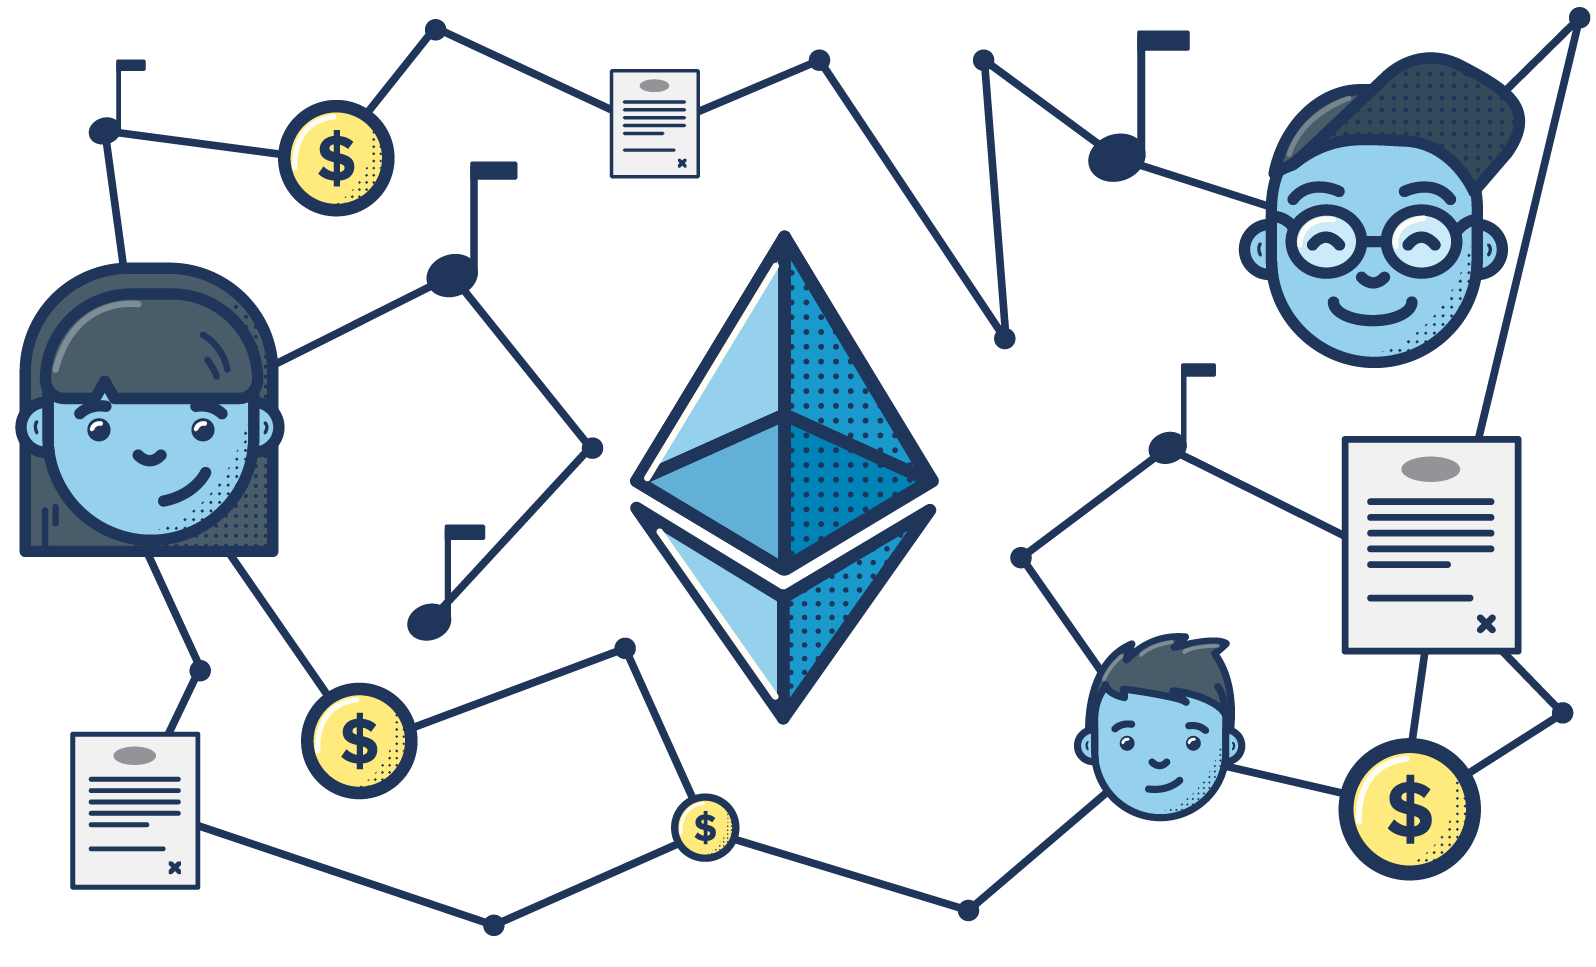
\includegraphics[width=0.60\textwidth]{figures/blockchain.png}
	\end{figure}
\end{frame}
\begin{frame}
	\frametitle{Excursus sulle Applicazioni Distribuite}
	\begin{figure}
		
\includegraphics[width=0.90\textwidth]{figures/truffle.png}
	\end{figure}
	\bigskip
	Su tale rete è possibile mettere a disposizione delle applicazioni che chiunque può utilizzare dietro pagamento di una piccola commissione. Queste applicazioni sono realizzabili dagli sviluppatori interessati tramite vari framework e suite di applicativi, il più celebre è \textbf{Truffle}.
\end{frame}
\begin{frame}
	\frametitle{Excursus su Git}
	Git è un software che permette in maniera semplice di gestire insiemi di file tramite un sistema di controllo di versione, una grande risorsa per gli sviluppatori che devono contribuire in maniera condivisa ad uno stesso progetto o che devono tenere sotto controllo i vari cambiamenti che sono stati apportati ai vari file e documenti.
	\begin{figure}
		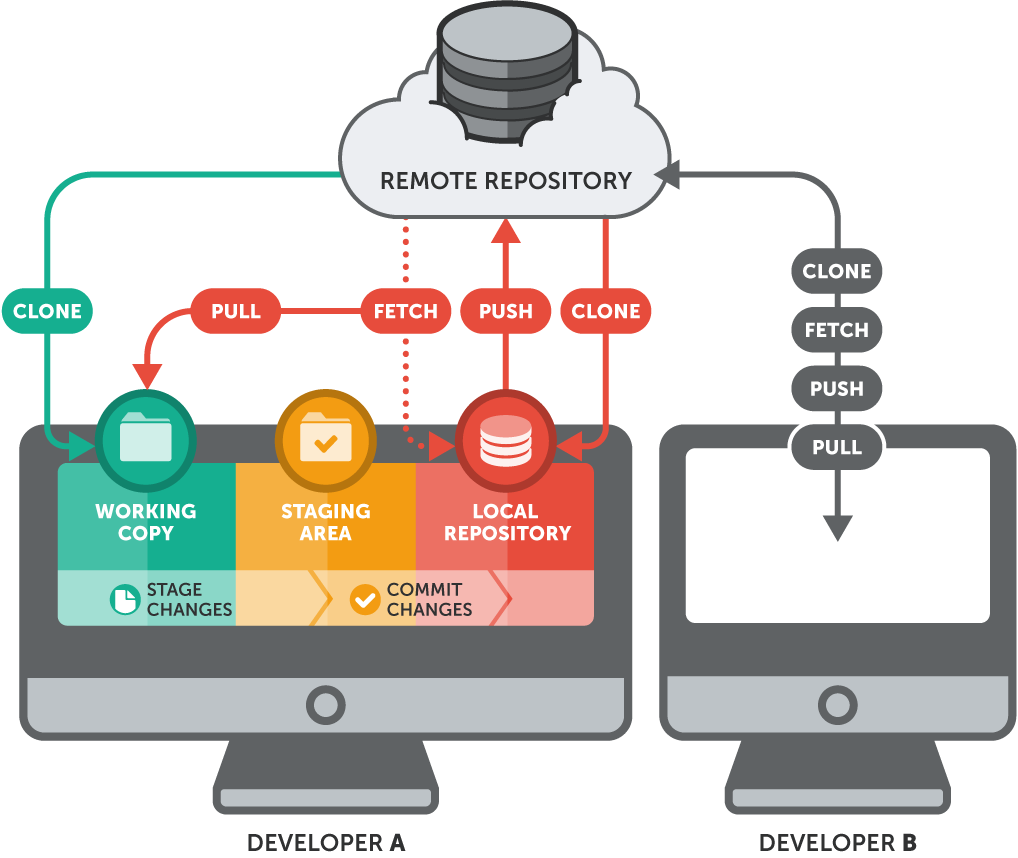
\includegraphics[width=0.45\textwidth]{figures/git2.png}
	\end{figure}
\end{frame}
\begin{frame}
	\frametitle{Excursus sulle funzioni di hashing}
	Funzioni non invertibili che permettono di associare in maniera univoca (o quasi) stringhe di caratteri (e quindi anche documenti di varia natura tradotti in stringhe) a delle stringhe alfanumeriche di lunghezza fissa.
	\bigskip
	\begin{figure}
		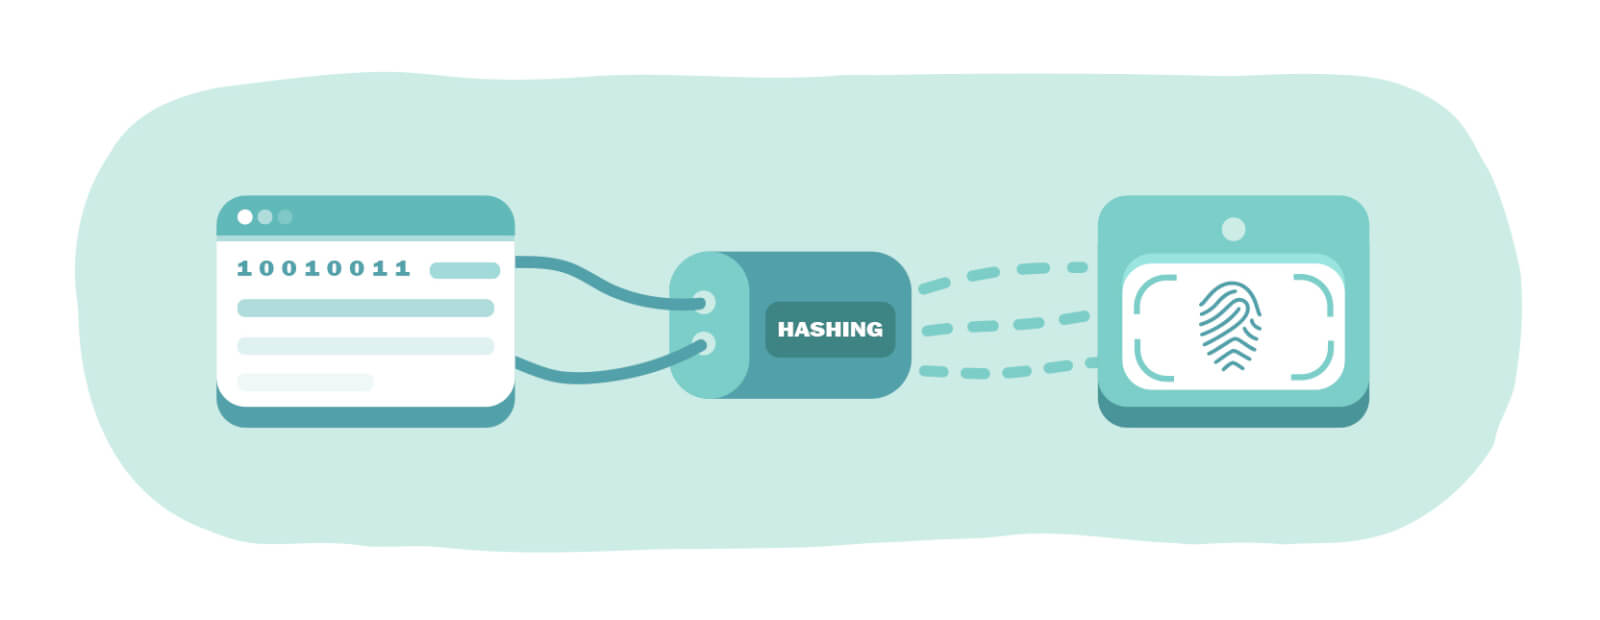
\includegraphics[width=0.85\textwidth]{figures/hashing.jpg}
	\end{figure}
\end{frame}
\section{Progettazione}
\begin{frame}
	\frametitle{Fase 4: Progettazione - Prima stesura}
	\begin{columns}
		\column{0.5\textwidth}
			La stesura iniziale è stata svolta dal professore che mi ha quindi fornito una linea guida da cui poter prendere spunto per poter realizzare il progetto dopo aver concordato sulle funzionalità del progetto, tale architettura è stata tuttavia modificata abbastanza in quanto le tecnologie utilizzate sono ancora troppo sperimentali e non offrono gli strumenti per potere essere adattati ad una struttura del genere.
		\column{0.5\textwidth}
		\begin{figure}
			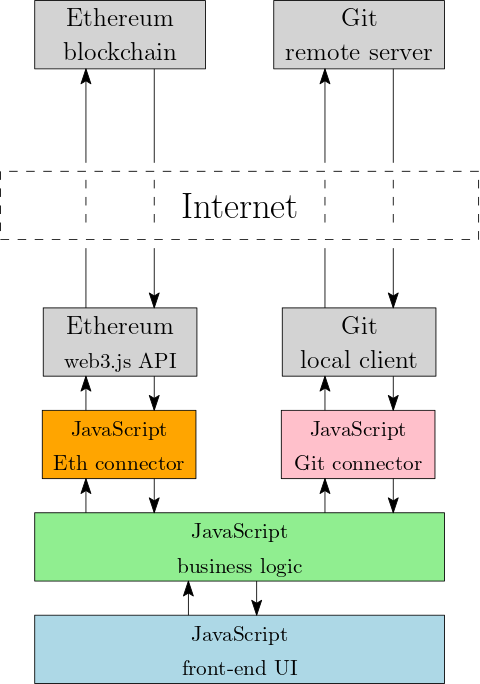
\includegraphics[width=0.88\textwidth]{figures/architecture1.png}
		\end{figure}
	\end{columns}
\end{frame}
\begin{frame}
	\frametitle{Fase 4: Progettazione - Seconda stesura}
	\begin{columns}
		\column{0.5\textwidth}
			\begin{figure}
				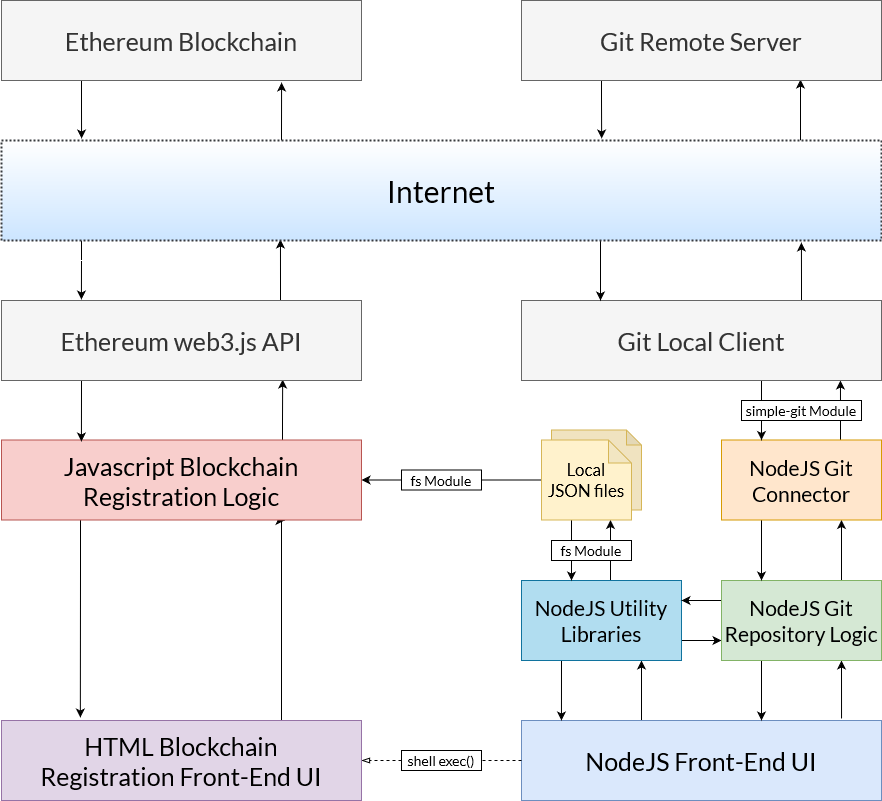
\includegraphics[width=1\textwidth, height=1.05\textwidth]{figures/architecture2.png}
			\end{figure}
		\column{0.5\textwidth}
		Il Front-End in NodeJS che comunica con una parte logica è stata mantenuta, sono stati però introdotti alcuni moduli Utility che vengono utilizzati da entrambe le componenti.

		La connessione alla Blockchain avviene attraverso l’avvio di un Web Server apposito e l’apertura di una scheda del browser, l’interazione da parte dell’utente deve avvenire tramite l’add-on Metamask.
	\end{columns}
\end{frame}
\section{Apprendimento}
\begin{frame}
	\frametitle{Fase 5: Apprendimento}
	In concomitanza con la fase di progettazione è stato necessario l’apprendimento di alcune tecnologie in modo da poter imparare le loro modalità di utilizzo e poter effettuare la seconda stesura dello schema progettuale.

	Oltre alla già citati suite Truffle e Metamask, abbastanza intuitivi nell'utilizzo, le tecnologie che seguono sono quelle che hanno occupato la maggior parte di questa fase.
	\begin{figure}
		
\includegraphics[width=0.50\textwidth]{figures/metamask.png}
	\end{figure}
\end{frame}
\begin{frame}
	\frametitle{Fase 5: Apprendimento - Solidity}
	\begin{columns}
		\column{0.5\textwidth}
		Per l’apprendimento della sintassi e delle peculiarità del linguaggio da utilizzare per scrivere DAPP per la Blockchain Ethereum mi sono avvalso della documentazione ufficiale e del tutorial interattivo \textbf{CryptoZombies}.	
		\column{0.5\textwidth}
		\begin{figure}
			
\includegraphics[width=0.30\textwidth]{figures/solidity.png}
		\end{figure}
		\begin{figure}
			
\includegraphics[width=0.40\textwidth]{figures/zombie.png}
		\end{figure}
	\end{columns}
\end{frame}
\begin{frame}
	\frametitle{Fase 5: Apprendimento - Javascript Asynchronous Programming}	
	\begin{figure}
		
\includegraphics[width=0.65\textwidth]{figures/async.jpg}
	\end{figure}
	L’utilizzo di alcuni moduli all’interno dell’applicazione ha richiesto che io spendessi diverso tempo ad imparare le tecniche di programmazione asincrona di Javascript in quanto lo scorretto utilizzo delle keyword async e await sono state fonte di svariati problemi nella prima fase della stesura del codice.
\end{frame}
\begin{frame}
	\frametitle{Fase 5: Apprendimento - Modulo Merkle Tree}
	\begin{columns}
		\column{0.5\textwidth}
		La necessità di dover calcolare una singola stringa Hash per una moltitudine di file ha portato il professore a proporre l’utilizzo di questa struttura, è stato quindi necessario da parte mia non solo comprenderne bene il funzionamento ma anche essere in grado di poter utilizzare al meglio i moduli che fornivano metodi per lavorare con questi particolari alberi.
		\column{0.5\textwidth}
		\begin{figure}
			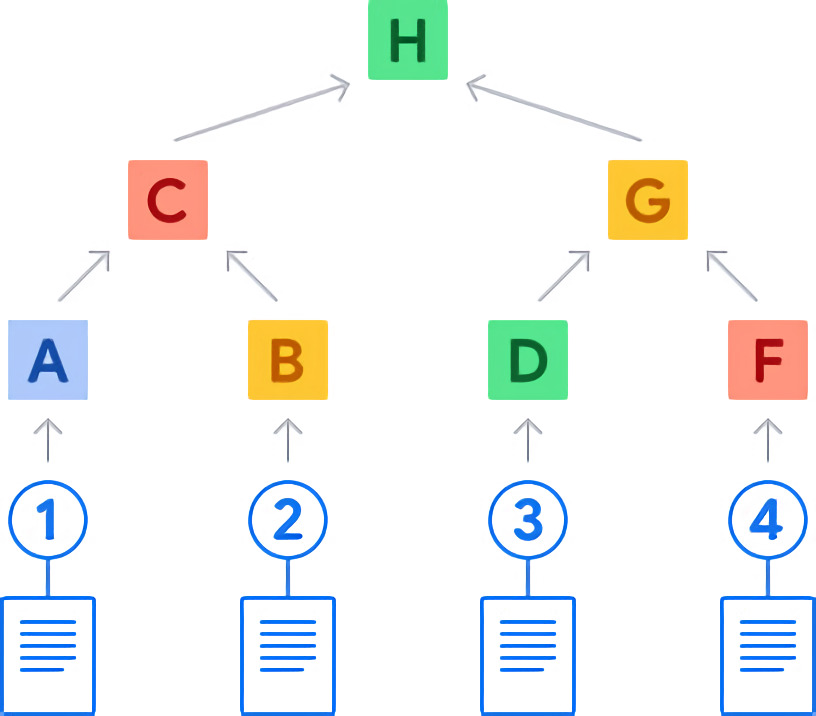
\includegraphics[width=0.88\textwidth]{figures/merkle-tree.jpg}
		\end{figure}
	\end{columns}
\end{frame}
\begin{frame}
	\frametitle{Fase 5: Apprendimento - Modulo InquirerJS}
	\begin{columns}
		\column{0.5\textwidth}
			\begin{figure}
				
\includegraphics[width=0.80\textwidth]{figures/inquirer.png}
			\end{figure}
		\column{0.5\textwidth}
		Anziché realizzare un Front-End dotato di GUI, ho preferito optare per una interfaccia testuale. Tuttavia, non volendo rinunciare all’immediatezza e la semplicità che un approccio grafico e user-friendly poteva portare al progetto ho imparato ad utilizzare il modulo di InquirerJS, il quale consente di realizzare menù con scelta a singola, multipla e libera in tutta comodità.
	\end{columns}
\end{frame}
\section{Implementa -zione}
\begin{frame}
	\frametitle{Fase 6: Implementazione}
	La fase di implementazione è divisibile in tre macro-sezioni:
	\begin{enumerate}
		\item Creazione delle librerie di utility e dei moduli di interfacciamento con Git
  		\item Creazione della CLI e del flow di interazione con le librerie e la logica di Git
  		\item Creazione del modulo di interrogazione e registrazione per la Blockchain
	\end{enumerate}
\end{frame}
\begin{frame}
	\frametitle{Creazione delle librerie di utility e dei moduli di interfacciamento con Git}
	La prima stesura di codice è avvenuta nella creazione della classe “connettore” per Git con il modulo “simple-git” e del relativo modulo Logic il quale richiama le sue funzioni a seconda della necessità della CLI.
\end{frame}
\begin{frame}
	\frametitle{Creazione delle librerie di utility e dei moduli di interfacciamento con Git}
	In concomitanza ho scritto i moduli del package “lib”:
	\begin{itemize}
		\item files: Lettura e scrittura di file JSON in cui conservare le informazioni riguardanti la Storage Unit o l’utente che sta utilizzando l’applicativo;
		\item inquirer: Contiene tutte le scelte che vengono poi presentate all’utente nella CLI;
		\item treelist: Si occupa di effettuare tutte le operazioni riguardanti l’hashing di file, l’assegnazione di hash alle subdirectories e la creazione e gestione di Merkle Tree.
	\end{itemize}
\end{frame}
\begin{frame}
	\frametitle{Creazione della CLI e del flow di interazione con le librerie e la logica di Git}
	Ho proseguito andando a creare l’effettivo workflow del programma richiamando le scelte dal modulo inquirer e funzioni differenti in base alle selezioni dell’utente.	
\end{frame}
\begin{frame}
	\frametitle{Creazione della CLI e del flow di interazione con le librerie e la logica di Git - Workflow}
	\begin{figure}
		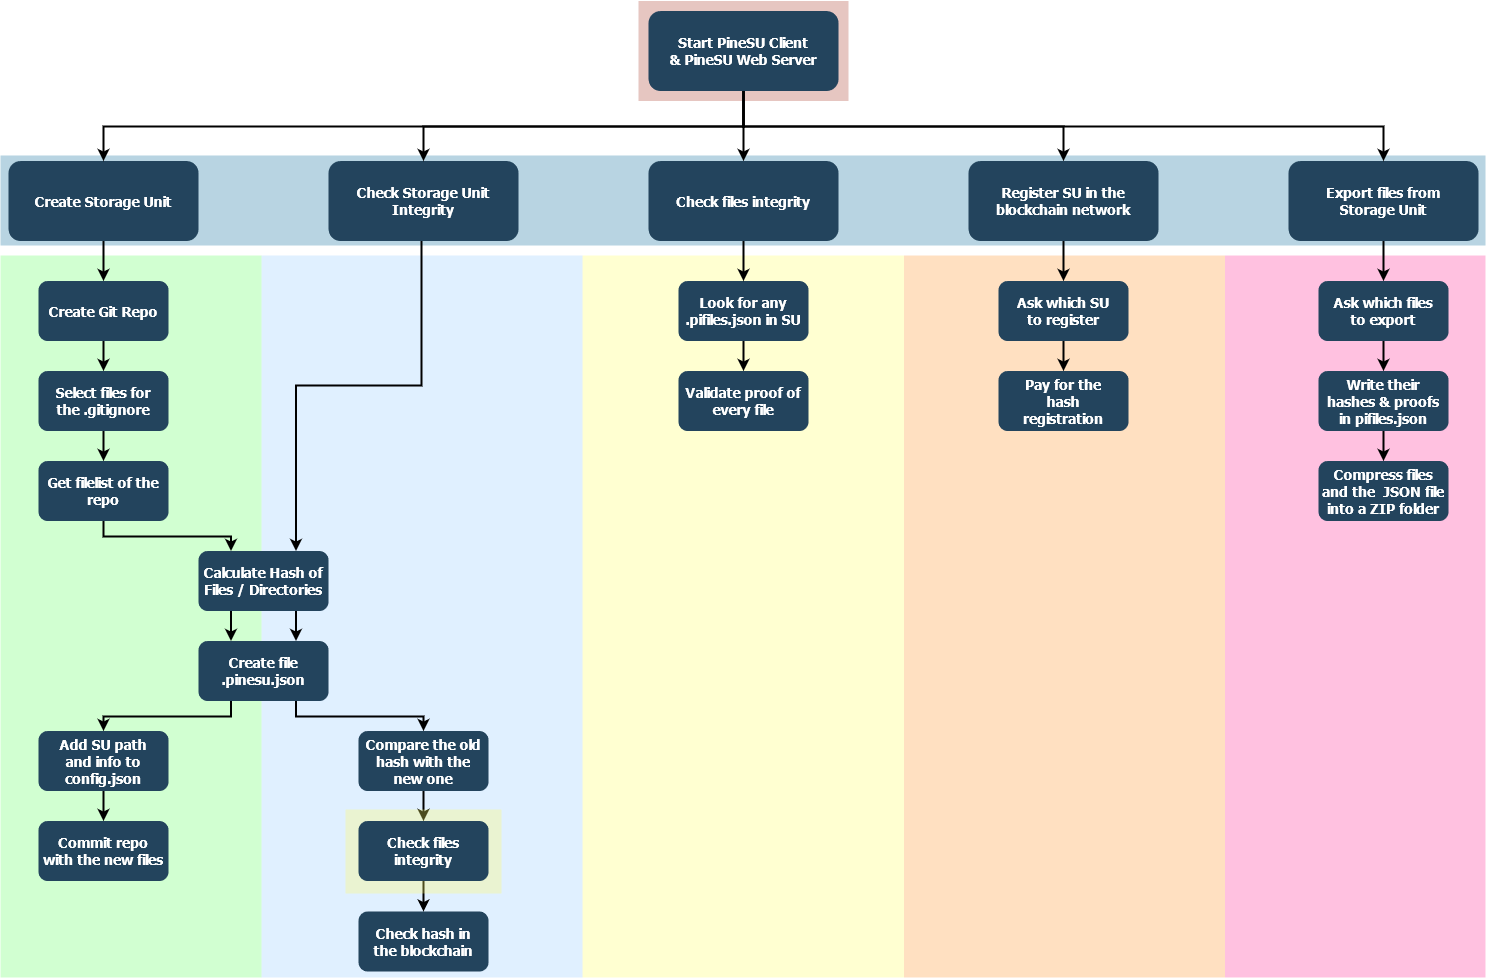
\includegraphics[width=1\textwidth]{figures/workflow.png}
	\end{figure}
\end{frame}
\begin{frame}
	\frametitle{Creazione del modulo di interrogazione e registrazione per la Blockchain}
	\begin{columns}
		\column{0.5\textwidth}
		\begin{figure}
			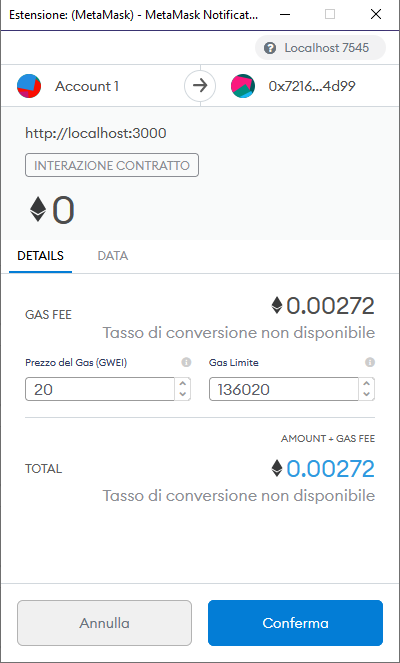
\includegraphics[width=0.6\textwidth]{figures/meta-gui.png}
			\caption{Transazione per registrare un hash nella blockchain}
		\end{figure}
		\column{0.5\textwidth}
		L’ultima parte della fase di implementazione è stata la realizzazione del Web Server locale che permette all’utente di registrare gli hash delle proprie Storage Unit nella blockchain, il risultato è stato ottenuta con una versione pesantemente modificata dell’applicazione di esempio fornita dal sito della suite Truffle.
	\end{columns}
\end{frame}
\section{Resoconto}
\begin{frame}
	\frametitle{Resoconto}
	\begin{itemize}
		\item Data di inizio tirocinio: 15/2/2020
  		\item Data di fine tirocinio: 28/5/2020
  		\item Totale Ore: 150 (25 ore \(\cdot\) 6 CFU)
  		\item Professore Tutor: Luca Grilli
  		\item Studente Tirocinante: Paolo Speziali
  		\item Anno Accademico: 2020/2021
	\end{itemize}
\end{frame}
\section{Fonti}
\begin{frame}
	\frametitle{Fonti}
	\begin{itemize}
		\item \href{https://ethereum.org/it/developers/}{Strumenti Ethereum per sviluppatori} 
  		\item \href{https://www.trufflesuite.com/tutorial}{Tutorial Truffle DAPPs - Pet Shop}
  		\item \href{https://www.sitepoint.com/javascript-command-line-interface-cli-node-js/}{Build a JavaScript CLI with Node.js}
  		\item \href{https://developer.mozilla.org/en-US/docs/Learn/JavaScript/Asynchronous/Async_await}{Tutorial di Mozilla su async / await}
  		\item Immagini reperite dai siti ufficiali degli strumenti eccetto per alcune scaricate da queste pagine web:
			\begin{itemize}
				\item \href{https://www.poeticoding.com/hashing-a-file-in-elixir/}{Funzioni di Hashing}
				\item \href{https://www.romatoday.it/attualita/concorso-rai-fiera-roma-norme-covid-19.html}{Concorso pubblico}
				\item \href{https://www.criptovalute24.com/ethereum-migliora-la-sua-blockchain-rialzo-del-5-4/}{Ethereum Blockchain}
				\item \href{https://blog.netsons.com/git-software-guida-facile/}{Git repository}
				\item \href{https://amerlin.keantex.com/programmazione-asincrona-con-async-await-parte-2/}{async / await}
				\item \href{https://transparency.dev/verifiable-data-structures/}{Merkle Tree}
			\end{itemize}
			\item \href{https://waifu2x.booru.pics/Home/index}{Strumento di upscaling delle immagini} 
	\end{itemize}
\end{frame}
\end{document}